\cleardoublepage


\chapter{Information Extraction From Text}
\label{ch:nlp}

As previously discussed, the problem of big data has become more relevant in the recent years.  This problem does not apply only to the ever growing amount of multimedia data created by smartphones but also to the growing presence of information in the form of news, corporate files, medical records, government documents, court hearing and social media. There is an ever increasing flood of information in an unstructured form. Natural Language Processing (NLP) is related to the usage of computation methods to process such data as a mode of communication used by humans.

``There are lot many processes involved in the pipeline of NLP. At the syntactic level, statements are segmented into words, punctuation (i.e.  tokens) and each token is assigned with its label in the form of noun, verb, adjective, adverb and so on (Part of Speech Tagging).  At the semantic level, each word is analyzed to get the meaningful representation of the sentence.  Hence, the basic task of NLP is to process the unstructured text and to produce a representation of its meaning.''  \cite{singh2018natural}.



Information Extraction (IE) from text is the process of extracting useful information from textual sources by implementing techniques of NLP. It can be defined as the act of efficiently and effectively analyze text and extract valuable and relevant knowledge from it in the form of structured information. ``The goal of IE is to extract salient facts about pre-specified types of events, entities, or relationships, in order to build more meaningful, rich representations of their semantic content, which can be used to populate databases that provide more structured input.'' \cite{singh2018natural}.

In this thesis, NLP is implemented to serve the purpose of creating an algorithm capable of extracting relevant information from a textual source. Furthermore, the algorithm must also be able to categorize the extracted data according pre-specified categories such as "locations" and "activities".

This chapter starts with an introduction to Natural Language Processing in section \ref{sec:nlp}. Section \ref{sec:num} explains the process of representing text in a numerical vector form while describing the concept of word embeddings. Static and contextualized word embedding models are discussed in section \ref{sec:static} and \ref{sec:context} respectively. An overview on some of the available NLP libraries is presented in section \ref{sec:libraries}.

\newpage
\section{Natural Language Processing}
\label{sec:nlp}

Natural language processing is a subfield of linguistics, computer science, information engineering and artificial intelligence, which is devoted to the engineering of computational models and processes to give the ability of human-like comprehension of texts/languages to computers. \cite{Khurana2018}  

Human language is extremely complex and rarely precise, to understand it is not only understand what words alone mean, but also how linking them together creates meaning. The nature of the human language makes NLP one of the most difficult tasks in computer science. 

Figure \ref{fig:nlp_class} shows the classification of NLP, which consists in two major components, Natural Language Understanding (NLU) and Natural Language Generation (NLG) \cite{Khurana2018}.  \par




\begin{figure}[htb]
    \centering
    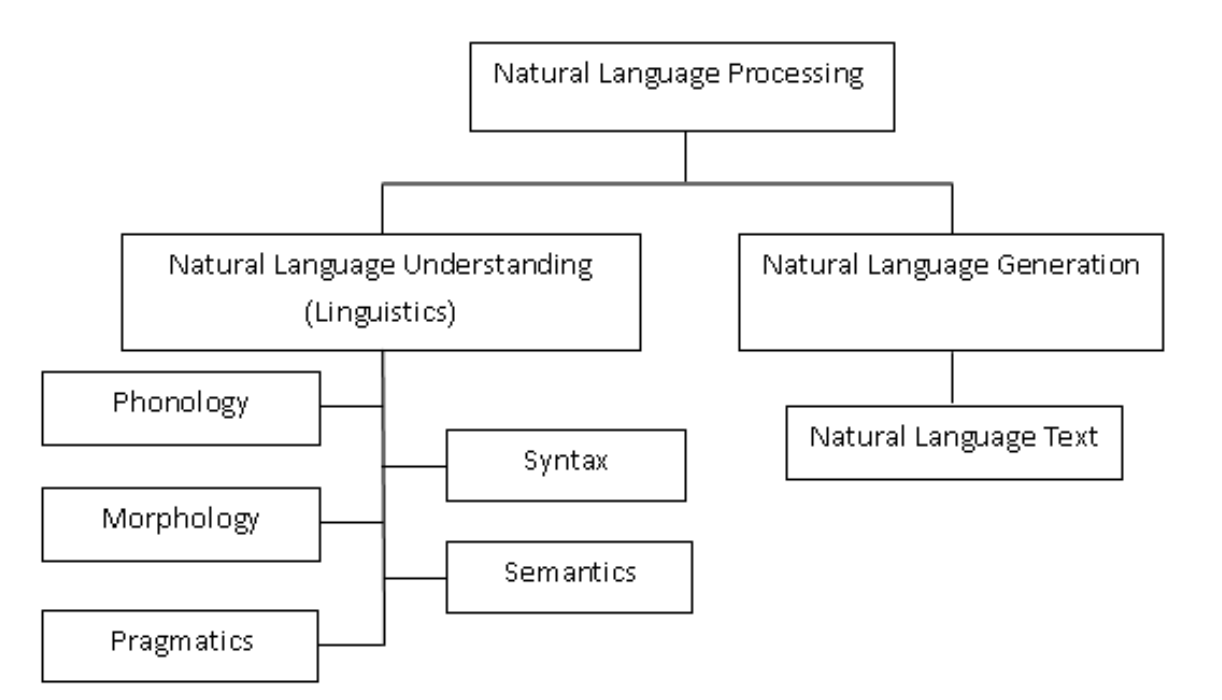
\includegraphics[scale = 0.3]{Sections/3StateOfTheArt/3_images/NLP_diagram.png}
    \caption{Classification of NLP \cite{Khurana2018}.}  
    \label{fig:nlp_class} 
\end{figure}

Natural Language Understanding is the process of understanding text. It is related to the science of Linguistic that studies the meaning of languages, context and various forms of language. 

Natural Language Generation is the process of generating text, sentences and
paragraphs that are meaningful from an internal representation \cite{Khurana2018}. 

Using the visual representation of Figure \ref{fig:nlp_class} the important terminologies of NLP are as follows \cite{Khurana2018} :

\begin{itemize}
    \item \textbf{Phonology}: The part of Linguistics which refers to the systematic arrangement of sound;
    \item \textbf{Morphology}: In linguistics, morphology is the study of words, how they are formed, and their relationship to other words in the same language. The different parts of the word represent the smallest units of meaning known as Morphemes;
    \item \textbf{Lexical}: In Lexical the focus is the interpretation of the meaning of individual words;
    \item \textbf{Syntax}: Syntax refers to the study of the grammatical structure of the sentence;
    \item  \textbf{Semantic}: Semantic processing determines the possible meanings of a
    sentence by pivoting on the interactions among word-level meanings in the sentence;
    \item \textbf{Discourse}: Discourse focuses on the properties of the text as a whole that convey meaning by making connections between component sentences;
    \item \textbf{Pragmatic:}: Subfield of linguistics that studies the ways in which the context of a sentence contributes to the meaning. 
    
\end{itemize}

The field of NLP can be divided in two broad sub-areas: core areas and application areas. The core areas address fundamental problems such as language modeling, morphological processing, parsing and semantic processing \cite{Otter2018}. 



\begin{itemize}
    \item Language modeling is considered the most important task in NLP and an essential piece in any application of NLP. It is the process of creating a model capable of predicting words or simple linguistic components given previous words or components. It can capture syntactic and semantic relationships among words or components in a linear neighborhood, making it useful for tasks such as machine translation and text summarization.
    \item Morphological processing is the process of finding segments within single words,  including roots and stems, prefixes and suffixes.
    \item Parsing examines how different words and phrases relate to each other.
    \item Semantic processing is the task of understanding of the meaning of words and phrases. This is done recurring to  word embedding models, like Word2Vec. This will be further discussed in this chapter.
\end{itemize}





The application areas address topics such as extraction of useful information from text (e.g named entities and relations), translation of text, summarization of written documents, automatic answering of questions, chat bots, email spam detection and many others \cite{Otter2018}.




\section{Numerical Representation of Text}
\label{sec:num}

\par Machine learning algorithms and most of all deep learning architectures are incapable of processing strings of text, this is because they require numbers as an input in order to perform linear algebra operations\cite{Vidhya2017} which is not possible with words. A human can easily tell that the word "dog" and the word "cat" are identical, since they both represent an animal, however a computer would assume that they are completely different things since all the letters in those  words are different. 

    \subsection{Word Embeddings}

    \par The dominant approach to solve this problem is the usage of word embeddings, which is a type of word representation that allows words with similar meaning to have a similar representation by mapping a set of words, or phrases in a vocabulary, to vectors of numerical values. For example, the word “happy” can be represented as a vector of 4 dimensions [0.24, 0.45, 0.11, 0.49] and “sad” has a vector of [0.88, 0.78, 0.45, 0.91]. The reason for this vectors to exist is so that a machine learning algorithm can perform linear algebra operations on numbers (vectors) instead of words \cite{MuratMustafa}. Word embedding methods learn a real-valued vector representation for a predefined fixed size vocabulary from a corpus  of text \cite{Brownlee2017}.A vector representation of a word may be a one-hot encoded vector where 1 stands for the position where the word exists and 0 everywhere else. 
    
    \par As an example, the sentence ”Word Embeddings are Word converted into numbers” can be converted to the following dictionary using the one-hot encoded vector representation : [‘Word’,’Embeddings’,’are’,’Converted’,"Word",’into’,’numbers’]. Using this representation the word “numbers” in the one-hot encoded vector is [0,0,0,0,0,1] and for the word "converted" is [0,0,0,1,0,0]. This is considered to be the most simple method to represent words in vector forms \cite{Vidhya2017}.

    \par The following image showcases the given example.
    
    
    \begin{figure}[htb]
        \centering
        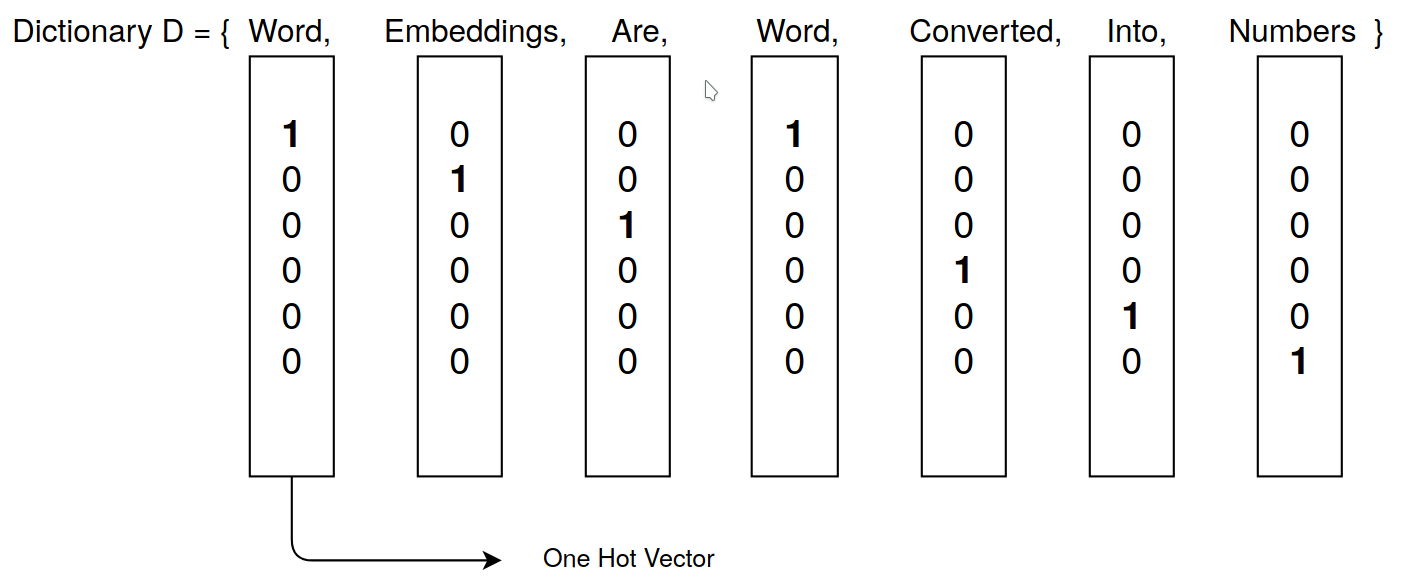
\includegraphics[scale = 0.23]{Sections/3StateOfTheArt/3_images/one_hot_encoding.png}
        \caption{Example of text representation by one-hot vector.}   
    \end{figure}
    
    
    



    \section{Static Word Embedding Models}
    \label{sec:static}

    \par This section introduces some common static word embedding models to learn word embeddings from text.


    \par Static word embedding have the fundamental problem which is they generate the same embedding, in different contexts, for the same word, failing to capture the polysemy of the word. This is due to the fact that each word has a single vector, regardless of context. \cite{Mikolov2013}  
   

    \par As an example, having these two phrases:

    \begin{itemize}
        \item "The Apple Company is the one who produces iPhones."
        \item "This apple is delicious."
    \end{itemize}

    \par In this case, the word "Apple" has two different meanings, being one a company and the other a fruit, however for static word embedding models, words only have one single meaning, and therefore  the word representation for "Apple" would be the same for both cases. \cite{Batista2018}

   
        \subsection{Word2Vec}

        \par Developed by Tomas Mikolov, et al.\cite{Mikolov2013} at Google in 2013, Word2Vec is a two-layer neural network that processes text by "vectorizing" words with the purpose of grouping vectors of similar words together in vectorspace. The way Word2Vec detects those similarities is by creating vectors that are distributed numerical representations of word features, without human intervention.


        \par In a regular one-hot encoded vector, all words have the same distance between each other, even though their meanings are completely different.



        \begin{figure}[H]
            \centering
            \captionsetup{justification=centering}
          
            \begin{subfigure}{0.32\textwidth}
            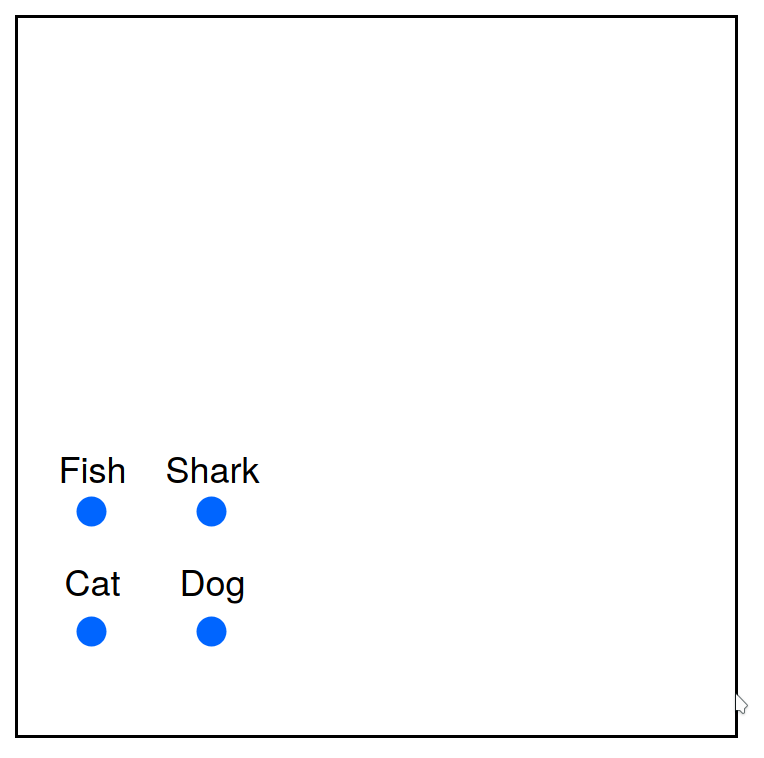
\includegraphics[width=\textwidth]{Sections/3StateOfTheArt/3_images/one_hot_ex.png} 
            \caption{One-hot encoding resulting vector. \cite{word2vec_explained}}
          
            \end{subfigure}
            \begin{subfigure}{0.32\textwidth}
            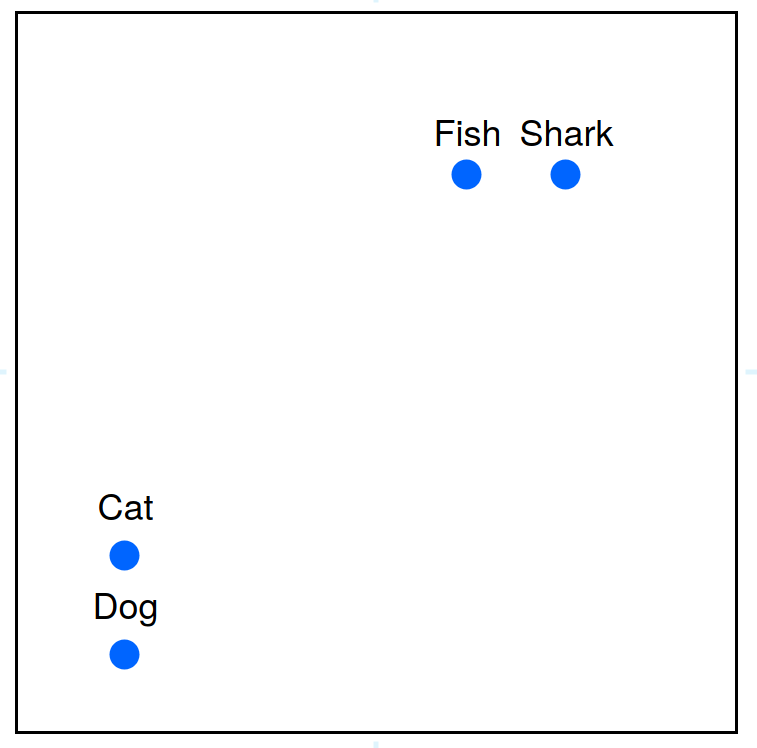
\includegraphics[width=\textwidth]{Sections/3StateOfTheArt/3_images/word2vec_encode.png}\hfill
            \caption{Word2Vec encoding resulting vector. \cite{word2vec_explained}}
            \end{subfigure}

          \end{figure}




        
        \par Word2Vec is capable of making accurate guesses, based on past appearances, of a word's meaning. 

        \par The output of Word2Vec is a vocabulary in which each item has a vector attached to it, which can be fed into a deep-learning net or simply queried to detect relationships between words.

        \par Word2Vec is composed of two different models, CBOW (Continuous Bag of words) which predicts a word given the context and Skip-Gram which predicts context given a word. \cite{Mikolov2013} \cite{Wiki}

        

        \begin{figure}[htb]
            \centering
            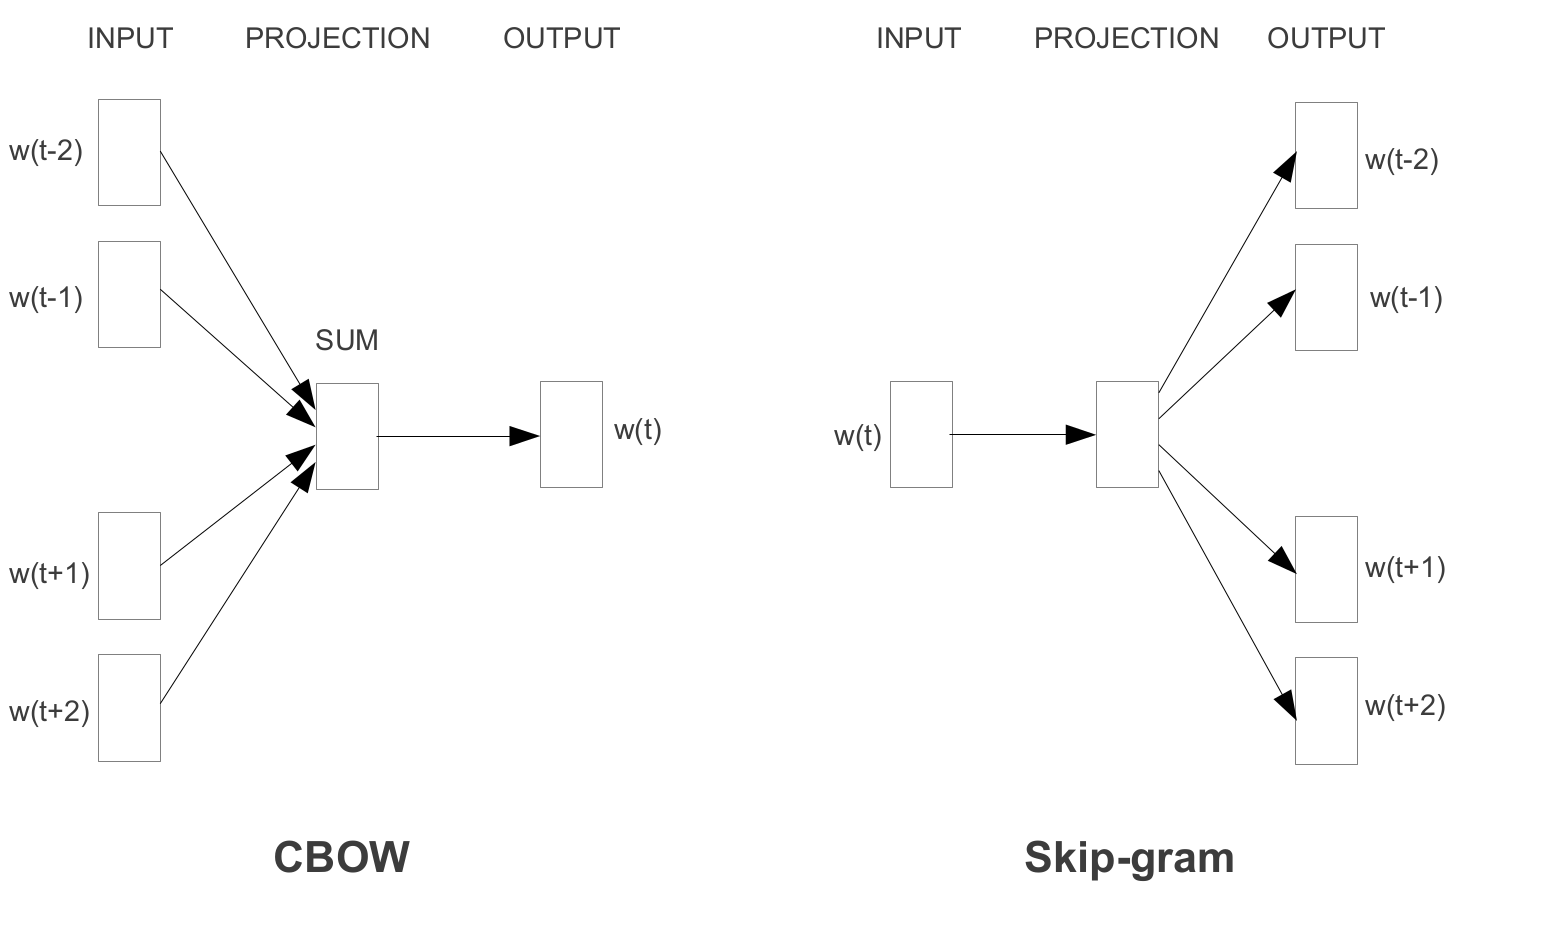
\includegraphics[scale = 0.15]{Sections/3StateOfTheArt/3_images/Cbow_Skip.png}
            \caption{CBOW model and Skip-Gram model. \cite{Mikolov2013}} 
        \end{figure}

        
        \subsection{GloVe}
            \par GloVe stands for Global Vectors for Word Representation and was a new approach created by Pennington et all. in 2014 \cite{Pennington2014} to generate word embeddings with unsupervised learning. Glove main goals are to create word vectors that capture meaning in the vector space and to take advantage of global count statistics instead of using only local information. 
            \par The problem with Word2Vec is that it only takes local information into account, and does not consider global context. This means that the semantics learnt for a given word are only affected by the surrounding words. 
            \par GloVe works by aggregating global word-to-word co-occurrence matrix from a of corpus text. This means that if two words keep appearing together in a corpus of text they either share a linguistic or a semantic similarity. Simply put, similar words will be placed together in the high-dimensional space. Therefore GloVe can be seen like an extension to the Word2Vec model.

        \subsection{FastText}

        \par FastText, created by Facebook's AI Research (FAIR) lab in 2016, is a fast text classifier based on the skipgram model  used for efficient learning of word representations and sentence classification. Popular models like word2Vec and GloVe  are based on continuous word representations that create vectors directly from words in a sentence while ignoring the morphology of words, this is done by assigning a distinct vector to each word, fastText uses a different approach treating each word as bag of characters n-grams. A vector representation is associated to each character n-gram and words are represented as the sum of these representations. This allows fastText to work with rare words not seen in the training data since the word is broken down into n-grams to get the corresponding embeddings \cite{bojanowski2016enriching}.


        \par Using the word "where" as an example and n=3, the representation of this word in a fastText model is <wh, whe, her, er, re> and the special sequence <where>. The angular brackets serve as boundary symbols to distinguish the n-gram of a word from the word itself, this means that if the word "her" was part of the vocabulary it would be represented as <her>, which allows the preservation of the meaning of shorter words and the understanding of suffixes and prefixes.

        

    
    \section{Contextualized Word Embedding Models}
    \label{sec:context}    
        \par Contextualized words embeddings aim at capturing word semantics in different contexts to address the issue of polysemous and the context-dependent nature of words \cite{Batista2018}. Using the example given in  section \ref{sec:static}, these models would be able to distinguish the different meaning of the word "apple" given the two different sentences.

        \subsection{Context2vec}
        
            \par Context2Vec is an unsupervised model capable of learning efficiently generic context embedding of wide sentential contexts, using a bidirectional LSTM. 

            A large plain text corpora is utilized in order to learn a neural model capable of embedding  entire  sentential  contexts  and  target words in the same low-dimensional space, which is optimized to reflect inter-dependencies between targets and their entire sentential context as a whole. 
            
            
            In contrast to word2vec that use context modeling mostly internally and considers the target word embeddings as their main output, the focus of context2vec is the context representation. Context2vec achieves its objective by assigning similar embeddings to sentential contexts and their associated target words \cite{Melamud2016}.

            \begin{figure}[htb]
                \centering
                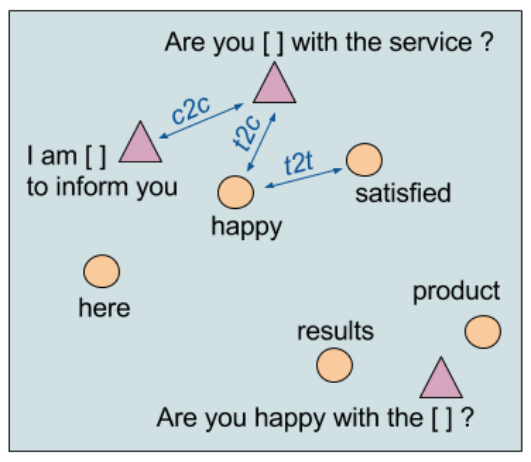
\includegraphics[scale = 0.35]{Sections/3StateOfTheArt/3_images/context2vec_embedding.png}
                \caption{A 2D illustration of context2vec’s embedded space and similarity metrics. Triangles and circles denote sentential context embeddings and target word embeddings, respectively \cite{Melamud2016}.} 
            \end{figure}

            \begin{figure}[htb]
                \centering
                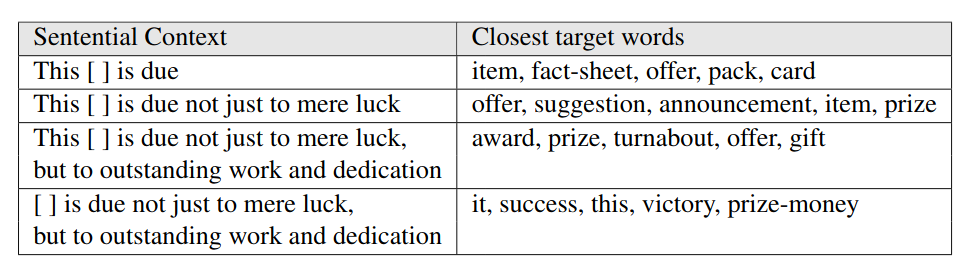
\includegraphics[scale = 0.35]{Sections/3StateOfTheArt/3_images/context2vec_predict.png}
                \caption{Closest target words to various sentential contexts, illustrating context2vec’s sensitivity to long range dependencies, and both sides of the target word \cite{Melamud2016}.} 
            \end{figure}
            
        \newpage


        \subsection{ELMo}

            \par ELMo (Embeddings from Language Models) is a NLP model with context-aware representation, it understands different meanings for the same word since it takes into account the surrounding words unlike traditional word embedding models such as Word2Vec and GLoVe. In order to achieve this, ELMo attributes an embedding for each word after looking at the entire context in which it is used, instead of using fixed embeddings for each word. Therefore, the same word might have different word vectors under different contexts.
            \par This NLP models both syntax and semantics of word use and how these uses vary across linguistic context.The word vectors are learned through the usage of internal states of a deep bidirectional LSTM algorithm, trained on a large corpus of text. Bidirectional implies that the algorithm takes into account the words before and the words after it in both directions. LSTM (Long Short-Term Memory) is one type of neural network that is able to retain data in memory for long periods of time, allowing it to learn longer-term dependencies.
            This language model can predict both the next word and the previous word and it is a character based model allowing the network to use morphological clues to form robust representations for out-of-vocabulary tokens not presented during training.  \cite{Peters:2018}
            \par Below an image showcasing an example of the differences between GLOVe that is a non-context aware model and ELMo biLM (bidirectional Language Model) that is context aware.

            
        \begin{figure}[htb]
            \centering
            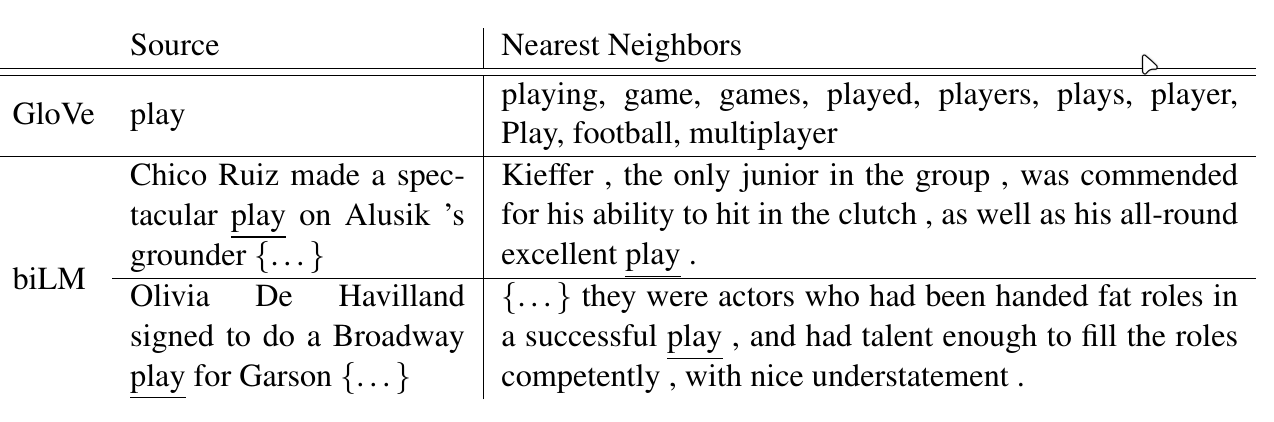
\includegraphics[scale = 0.3]{Sections/3StateOfTheArt/3_images/ELMO.png}
            \caption{Nearest neighbors to "play" using GLoVe and context embeddings from a biLM \cite{Peters:2018}.} 
        \end{figure}

        \par GLoVe only uses the word "play" as source, therefore the obtained neighbors for that word are spread across several parts of speech however they all focus on the sports-related sense of the word "play". ELMo biLM uses the entire sentence as source, this means that it is able to understand the context of the word, therefore in both cases, the biLM is able to disambiguate both the part of speech and word sense in the source sentence \cite{Peters:2018}.
        

       
\section{Available NLP libraries}
    \label{sec:libraries}

        \subsection{SpaCy}
        
        \par SpaCy is a free, open-source library for advanced natural language processing written in Python and Cython published by Explosion AI. It was designed specifically for production use and to help in the building of applications that process and "understand" large volumes of text data.  Some use cases for this specific library are to build information extraction or natural language understanding systems, or to pre-process text for deep learning. \cite{Spacy2017}

        \par This NLP library was chosen for the development of the text processing phase of the practical work, not only because ig provides a well written documentation and being simple to use but also because it offers many useful features such as:

        \begin{itemize}
            \item \textbf{Tokenization} : The segmentation of text into words, punctuation, etc
            \item \textbf{Part-of-Speech Tagging} : The assignment of word types to tokens, like verb, noun, etc
            \item \textbf{Similarity} : The comparison between different words, phrases or text documents and how similar they are.
            \item \textbf{Lemmatization} : The assignment of base forms of words.
        \end{itemize}

      

        \subsection{Natural Language ToolKit}

        \par Developed by Steven Bird, Edward Loper and Ewan Klein in the Department of Computer and Information Science at the University of Pennsylvania, NLTK (Natural Language ToolKit) is a suite of open source program modules, tutorials, problem sets and a leading platform for building Python programs to work with human language data. NLTK covers symbolic and statistical natural language processing, and is interfaced to annotated corpora. This library provides easy-to-use interfaces such as WordNet, along with a suite of text processing libraries for classification, tokenization, stemming, tagging, parsing, and semantic reasoning \cite{Loper2002}. 

        \subsection{Stanford Core NLP}

        \par Developed at Stanford University, Core NLP is library written in Java, however with wrappers for different languages, including Python. This library is fast and some of its components can be integrated to NLTK which boosts efficiency. CoreNLP enables users to derive linguistic annotations for text, including token and sentence boundaries, parts of speech, named entities, numeric and time values, dependency and constituency parses, coreference, sentiment, quote attributions, and relations \cite{Manning2015}.


        \subsection{Gensim}

        \par Gensim ("Generate Similar”) is a Natural Language Processing open-source library for unsupervised topic modeling (a technique to extract the underlying topics from large volumes of text)  and for natural language processing. This python-cython library specializes in finding the semantic similarity between two documents through vector space modeling and topic modeling toolkit. It is capable of building document or word vectors, corpora, performing topic identification, performing document comparison (retrieving semantically similar documents) and analysing plain-text documents for semantic structure. In terms of producing word embedding, gensim allows for the usage of Word2Vec and fastText \cite{rehurek_lrec}.

        
        \subsection{Uncommon Libraries}
        Other NLP libraries not so common are Flair \cite{akbik2018coling}, Polyglot \cite{polyglot:2013:ACL-CoNLL}, CogCompNLP \cite{2018_lrec_cogcompnlp}, TextBlob \cite{textblob}.